\documentclass[11pt]{standalone}
 
\usepackage{tikz}
\usepackage{pgfplots} 
\usepackage{xcolor}
\usepackage{tabularx}
\pgfplotsset{width=6.05cm,compat=newest}

\newcommand{\tab}[1][1cm]{\hspace{#1}}
\pgfplotsset{
  /pgfplots/colormap={pink}{%
    color(0cm) = (purple);
    color(1cm) = (pink!80!purple);
    color(2cm) = (pink!90);
    color(3cm) = (pink) }
}
\newcommand\placeheart[1]{
  \begin{tikzpicture}
    \begin{axis}[
        view={0}{10}, 
        axis equal,
        axis lines=none,
        colormap name =pink, 
        scale=1.6
      ]
      \addplot3[
        surf,
        shader=faceted,
        samples=#1,
        domain=0:2*pi,y domain=0:2*pi,
        z buffer=sort,
        opacity=0.35
      ] 
      (
        {(sin(deg(x)))^3*cos(deg(y))},
        {(sin(deg(x)))^3*sin(deg(y))},
        {(13*cos(deg(x))-5*cos(2*deg(x))-2*cos(3*deg(x))-cos(4*deg(x)))/16}
      );
    \end{axis} 
  \end{tikzpicture}
}
\begin{document}
%\begin{tabularx}{20cm}{XXXXX}
%  \placeheart{5} && \placeheart{8} && \placeheart{10} \\
%    & \placeheart{15} && \placeheart{25} &\\
%   && \placeheart{40} &&
%\end{tabularx}
\newcommand{\hatgraph}[1]{
  \begin{tikzpicture}
    \begin{axis}[
        hide axis,
        colormap/violet,
    ]
    \addplot3[
        surf,
        samples=#1,
        shader=faceted,
        domain=-8:8,
        opacity=0.8
    ]
    {sin(deg(sqrt(x^2+y^2)))/sqrt(x^2+y^2)};
    \end{axis}
    \end{tikzpicture}
}
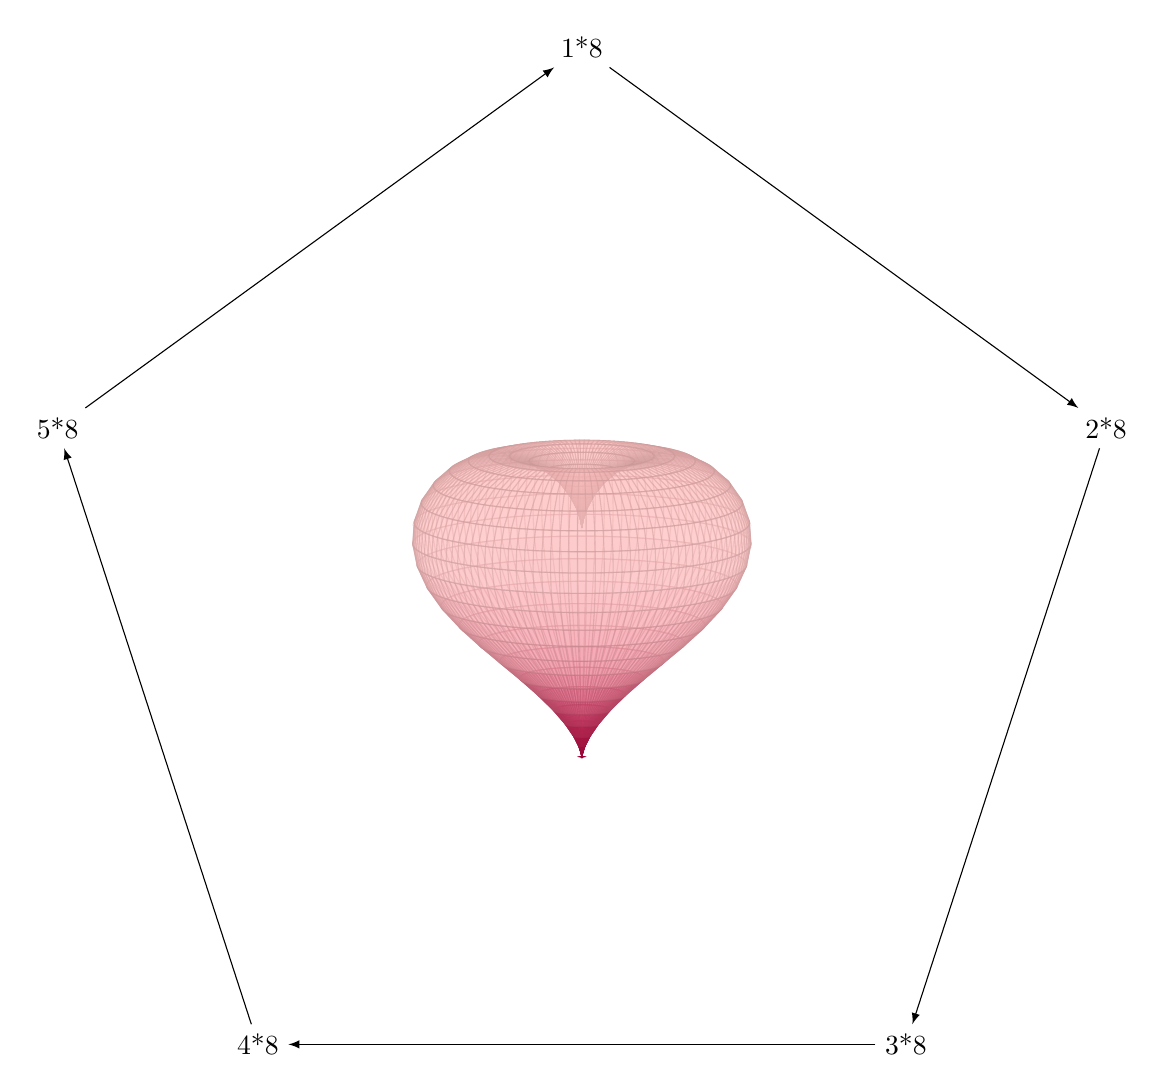
\begin{tikzpicture}
\foreach \x in {1,...,5}{
  \node (\x) at(162-\x*72:7cm) {
    \hatgraph{\x*8}
  };
}
\node at(0,0) {\placeheart{60}};
\draw[-latex] (1) -- (2);
\draw[-latex] (2) -- (3);
\draw[-latex] (3) -- (4);
\draw[-latex] (4) -- (5);
\draw[-latex] (5) -- (1);
\end{tikzpicture}

  
\end{document} 
